\subsection{Giao diện quản lý thành viên trong workspace}

\begin{figure}[H]
    \centering
    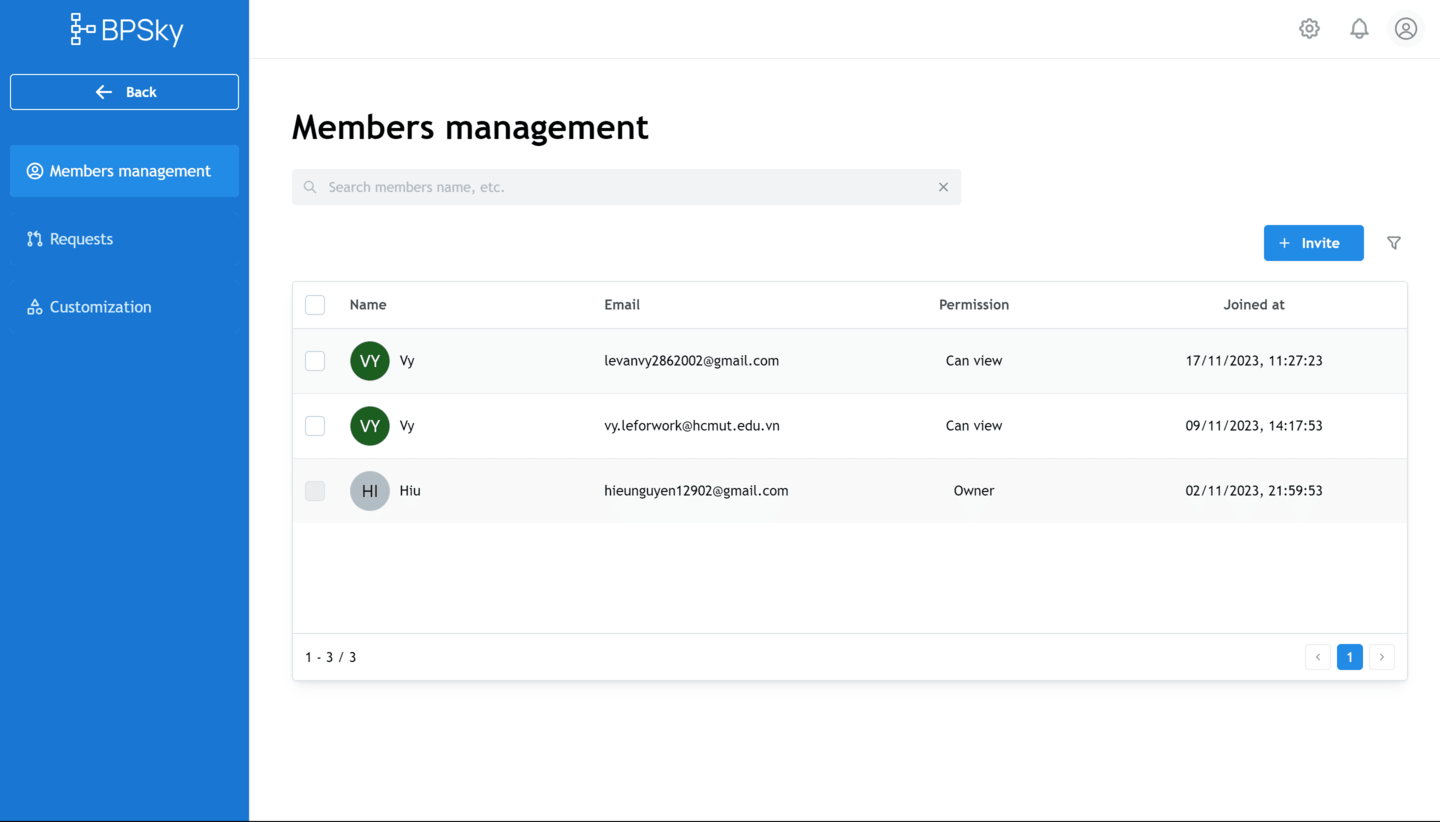
\includegraphics[ width = 0.8\linewidth]{Content/Hiện thực hệ thống/documents/Hiện thực giao diện người dùng/images/MembersManagementPage.png}
    \vspace{0.5cm}
    \caption{Giao diện trang quản lý thành viên trong Workspace}
    \label{fig: Giao diện trang quản lý thành viên trong Workspace}
\end{figure}

Nếu người dùng là người sở hữu workspace (workspace owner) thì có thể chọn icon bánh răng bên cạnh tên của workspace tại trang Workspace Detail để điều hướng tới giao diện quản lý workpsace. Người dùng sẽ được điều hướng mặc định tới trang quản lý thành viên trong workspace. Hệ thống sẽ hiển thị danh sách những thành viên có trong workspace cùng với quyền hạn và thời gian tham gia workspace của họ, chúng ta có thể lọc người dùng theo vai trò trong hệ thống. Nếu người sở hữu workspace muốn mời thêm thành viên trong hệ thống vào workspace thì có thể chọn nút "Invite", hệ thống sẽ mở Share modal - Share modal này sẽ gửi lời mời trực tiếp đến người dùng thông qua hòm thông báo.